\chapter{Conceptos previos}
\label{cap:conceptos}

\section{Impresoras 3D}
\label{sec:immpresoras}

En los últimos años ha tenido un gran auge las denominadas impresoras 3D. Máquinas capaces de crear un objeto físico de cero mediante un proceso de fabricación aditiva. Este tipo de fabricación está siendo una nueva revolución, de igual manera que pasó hace unos años con la conocida web 2.0, en la que el usuario era capaz de generar contenido para la propia página. Con la fabricación aditiva, pasaremos de la fabricación 1.0 (producción de objetos físicos por grandes empresas y expertos) a la fabricación 2.0 (producción de los objetos por el cliente final) \cite{additive}.\\

La fabricación aditiva es una colección de procesos que unen materiales para crear objetos físicos en 3D directamente desde un diseño en ordenador. Estos procesos, se caracterizan en que van añadiendo distintas capas que conforman el elemento final (ver figura \ref{fig:approach_am}), que es todo lo contrario al mecanizado, en la que se conforma la pieza por eliminación de material, ya sea por arranque de viruta o por abrasión.\\

Una de las ventajas de la fabricación aditiva es su rapidez \cite{additivevssubtractive}, dependiendo de la complejidad de la pieza puede suponer un par de horas de fabricación, frente a una jornada completa de trabajo con las máquinas de mecanizado. Por ello, también se conocen a este tipo de máquinas, como máquinas de prototipado rápido.\\

\begin{figure}[H]
    \centering
    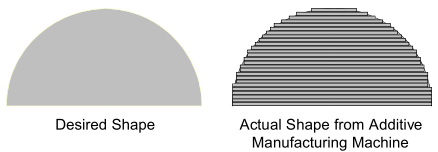
\includegraphics[width=0.6\textwidth]{images/aproximacion_am.png}
    \caption[Aproximación de una pieza con fabricación aditiva.]{Aproximación de una pieza con fabricación aditiva. A la izquierda podemos observar la forma final deseada. A la derecha la forma final obtenida y como la pieza está formada por un número determinado de capas. Fuente \cite{additive}}
    \label{fig:approach_am}
\end{figure}

Antiguamente, cuando sólo las grandes empresas disponían de ordenadores y se quería hacer algún tipo de cálculo numérico o tratamiento de información, era necesario ir a los centros de cálculos con los datos requeridos, para que, después de días o incluso semanas, obtener nuestros resultados y en el mejor de los casos, haber realizado correctamente el ensayo y no tener que volver a repetirlos, si los resultados no eran los deseados, se debería volver a repetir la operación.\\

Con la fabricación de las piezas pasa algo similar. En el caso de que quisiéramos diseñar alguna pieza para cubrir nuestras necesidades, debíamos acudir a empresas que dispusieran de las máquinas necesarias para tratar los materiales, y pasado cierto tiempo tendríamos la pieza. Una vez en nuestro poder, deberíamos comprobar que la pieza cumple con nuestras especificaciones y ver que no nos equivocáramos a la hora de tomar alguna medida y saber las tolerancias de la máquina. Gracias a la tecnología aditiva, el tiempo se ha acortado, y como veremos más adelante, a día de hoy, no es necesario acudir a ninguna empresa para poder realizar nuestras propias piezas.\\

La tecnología aditiva lleva muchos años usándose y sin embargo no ha sufrido muchos cambios desde que empresas como 3D Systems, Stratatasys o incluso el MIT, la usaran a mediados de los años 80. A pesar de ello, no ha sido hasta hace unos pocos años (2009) cuando la tecnología ha llegado al público en general. Se debe a que el funcionamiento de este tipo de tecnologías estaban protegidas por patentes. La principal patente es la que desarrolló \textbf{S. Scott Crump} co-fundador de Stratasys \cite{crump1992apparatus}, la cual expiro en 2009 y permitió que pudiera extenderse el uso de esta tecnología. En la figura \ref{fig:impr_patente_sistema} podemos ver una imagen extraida de la patente.\\

\begin{figure}[H]
    \centering
    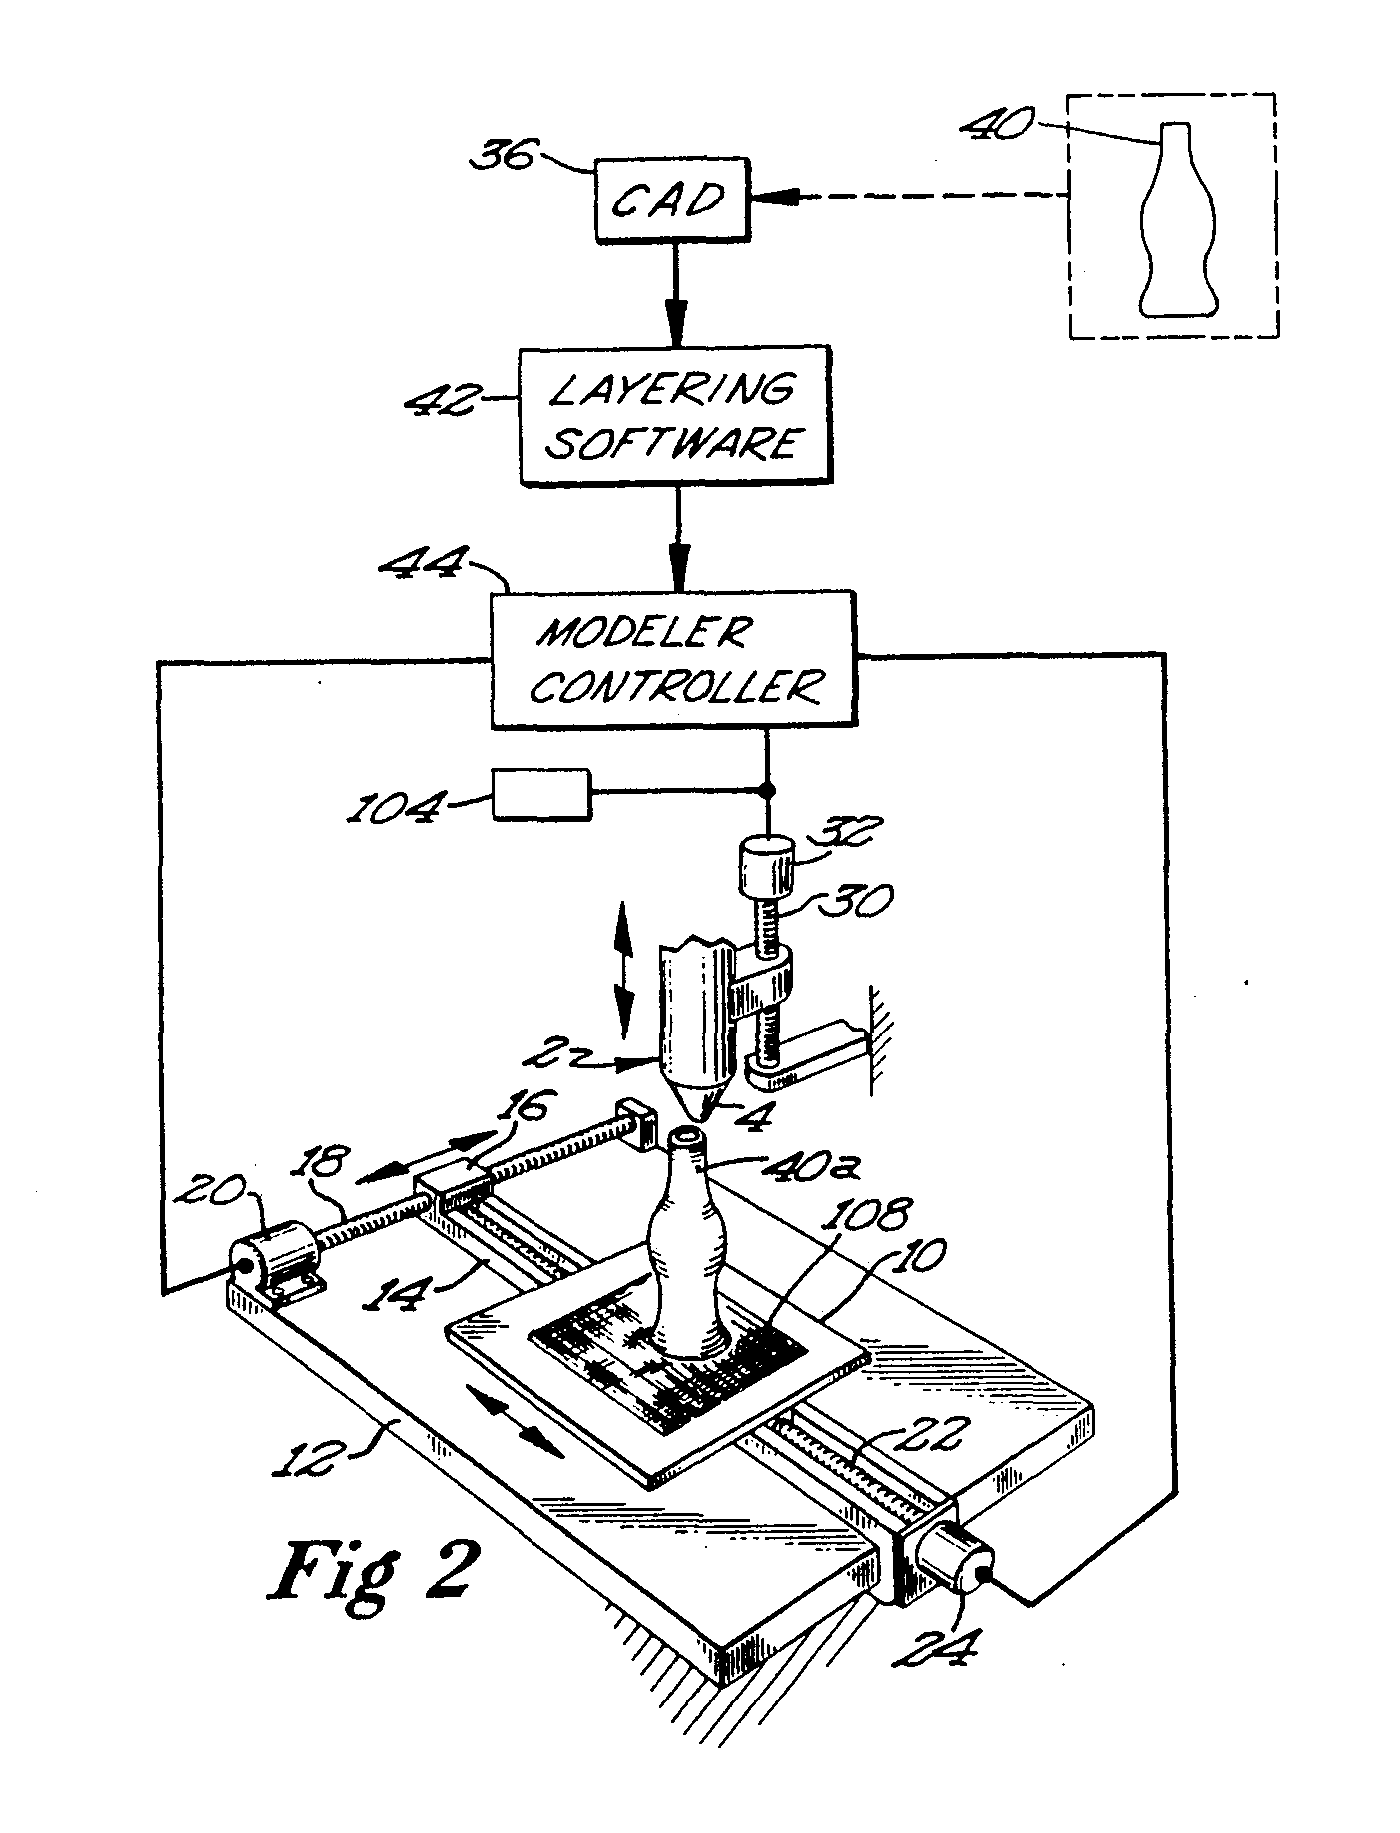
\includegraphics[width=0.6\textwidth]{images/estado.arte/US5340433-2.png}
    \caption[Esquema de la patente de S. Scott Crump.]{Esquema de la patente de S. Scott Crump en el que se detallan los distintos elementos que conforman un sistema capaz de fabricar un modelo físico a partir de un diseño generado por ordenador Fuente  \cite{crump1992apparatus}}
    \label{fig:impr_patente_sistema}
\end{figure}


\section{Fabricación de modelado por deposición fundido}
\label{sec:FDM}
La fabricación de modelado por deposición fundido (en inglés FDM\textregistered ) es la tecnología aditiva que más se ha popularizado en los últimos años. Aunque estas siglas están registradas por la empresa Stratasys Inc. ya que su co-fundador,  \textbf{S. Scott Crump} fue quien desarrollo está tecnología. Por ello, se usa el término equivalente, fabricación con filamento fundido (\textbf{FFF}).\\  

En la figura \ref{fig:impr_fdm} podemos ver en detalle el principio de funcionamiento de este tipo de impresoras. La máquina dispone de un elemento fusor (1), que está por encima de la temperatura de transición vítrea del polímero, haciendo que entre en un estado viscoso y maleable. El fusor deposita el polímero (2) en distintos niveles sobre una superficie plana (3) a la vez que se desplaza en los tres ejes cartesianos (X,Y,Z), de este modo, la pieza es creada con el filamento que solidifica al salir del fusor.\\

\begin{figure}[H]
    \centering
    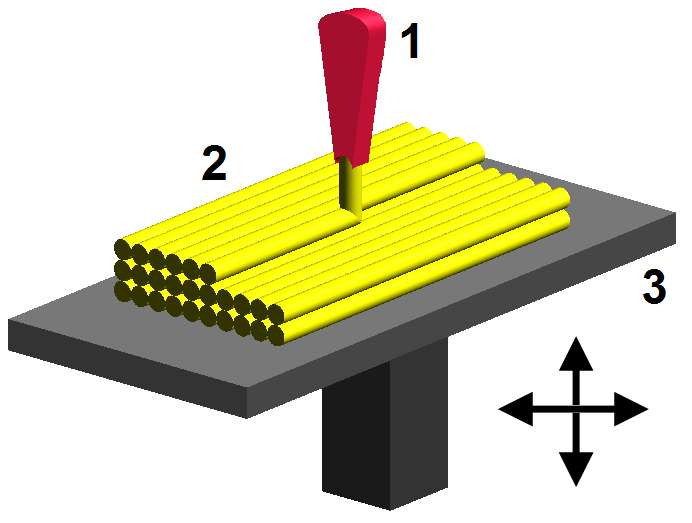
\includegraphics[width=0.4\textwidth]{images/FDM_by_Zureks.png}
    \caption[Principio de la fabricación con filamento fundido]{Principio de la fabricación con filamento fundido. (1) Elemento fusor o extrusor. (2) Polimero fundido. (3) Superficie capaz de desplazarse en los tres ejes carterianos. Fuente \cite{fundamentoFDM}}
    \label{fig:impr_fdm}
\end{figure}

Este sistema de fabricación, tiene tres pasos definidos:

\begin{itemize}
    \item \textbf{Pre-procesado:} Un software especial lamina en capas y calcula las trayectorias necesarias para crear el objeto que queremos fabricar.
    \item \textbf{Producción:} La impresora 3D calienta el termoplástico hasta alcanzar un estado viscoso y maleable y lo va depositando en capas muy finas siguiendo las trayectorias anteriormente calculadas por el software. En los sitios en los que es necesario un soporte, el software laminador hace que se incorpore material que hará de sustento para el plástico que quede al aire, el cual será quitado de la pieza final.
    \item \textbf{Post-procesado:} Una vez que la impresora termina, la pieza será usable. En caso de haber puesto material, el usuario deberá removerlo antes de poder dar la pieza por terminada.
\end{itemize}

El modelo en 3D que se quiera construir, primero deberá ser diseñado con un programa CAD (Computer Aided Design) el cual, será exportado en un fichero con formato STL (StereoLithography). Un fichero STL es una representación triangular de una geometría en 3D. La superficie es dividida en una serie de triángulos orientados denominadas caras. Cada cara, es definida por una normal y tres puntos \cite{stl}. Sin embargo, este fichero no puede ser interpretado por una máquina FFF ya que lo único que entiende son coordenadas.\\

Por ello, el fichero STL deberá ser tratado por un programa laminador que divida el modelo 3D en distintas capas (ver figura \ref{fig:detalle_capas}) y genere las trayectorias necesarias para realizar cada capa. Este programa, almacenará las trayectorias en un lenguaje que se denomina G-code, que es comúnmente usado en control numérico (CNC), el cuál dirá a la impresora cómo hacer la pieza deseada.

\begin{figure}[H]
    \centering
    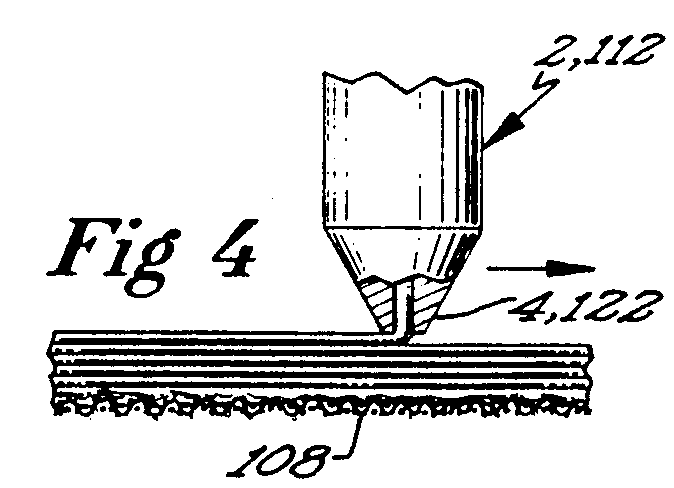
\includegraphics[width=0.4\textwidth]{images/capas_fdm.png}
    \caption[Detalle  de un extrusor realizando una pieza.]{Detalle  de un extrusor realizando una pieza.(2,112) Parte caliente por la que pasa el filamento y es fundido. (4,122) Boquilla por la que sale el filamento. (108) Distintas capas que conforman la pieza final. Fuente \cite{crump1992apparatus}}
    \label{fig:detalle_capas}
\end{figure}

Según explica Stratasys en su página web \cite{FDMTechnology}, la tecnología FFF tiene varios beneficios que la hacen idónea para fabricar:

\begin{itemize}
    \item La tecnología es limpia y fácil de usar por el usuario.
    \item Los termoplásticos usados son estables mecánicamente y con el medio ambiente.
    \item Formas complejas que con otra tecnología serían costosas de fabricar, con FFF son mucho más practicas de realizar.
\end{itemize}

Haciendo una traducción libre en la patente de S. Scott Crump \cite{crump1992apparatus} una impresora FDM es:

\begin{quotation}
    \emph{
    Aparato que incorpora un cabezal móvil dispensador (provisto de un suministro de material que solidifica a una temperatura predeterminada) y una base, los cuales se mueven relativamente entre sí a lo largo de los ejes “X”, “Y” y “Z” siguiendo un patrón predeterminado para crear objetos tridimensionales mediante la deposición controlada de material descargado desde el cabezal móvil sobre la base. El aparato está preferiblemente controlado por ordenador en un proceso que emplea software de diseño y fabricación asistido por ordenador (CAD-CAM) para generar señales de control y accionar el movimiento controlado del cabezal y la base mientras el material se está depositando.}\\

    \emph{La creación de objetos tridimensionales es posible mediante la deposición repetida de  capas de material de solidificación hasta alcanzar la forma deseada. Son susceptibles de uso materiales que se adhieran a la capa anterior con una unión adecuada tras la solidificación; tales como: ceras autoendurecibles, resinas termoplásticas, metales fundidos, epoxis bicomponentes,espumas y vidrios. La base de cada capa se define por la capa anterior, y el grosor de capa se define y controla mediante la altura a la que la punta del cabezal móvil está situada sobre la capa precedente}

\end{quotation}

\section{Materiales usados en impresión 3D}
\label{sec:materiales}

En la actualidad hay multitud de materiales que se pueden usar en las impresoras 3D. Siendo la mayoría de ellos polímeros termoplásticos, ya que si se les aplica una temperatura alta se vuelven deformables y al enfriarlos, pasando por un estado de transición vítrea, se endurecen.\\

Algunos materiales que se usan son:
\begin{itemize}
    \item Acrilonitrilo Butadieno Estireno o \textbf{ABS}.
    \item Poliácido Láctico o \textbf{PLA}.
    \item Alcohol de Polivinilo o \textbf{PVA} 
    \item \textbf{NYLON.}
\end{itemize}

Todos ellos tienen características que hacen idóneo su uso en diferentes campos. Por ejemplo, el ABS tiene unas propiedades mecánicas mejores que el PLA \cite{tfg_antonio}. Todos los polímeros comparten la propiedad que tienen una temperatura de fusión, relativamente baja, por lo que no es necesario un aporte de calor eleveado. Por ello, en función de la utilidad que se vaya a dar a la pieza final, será recomendable usar un polímero u otro.\\

Todos estos consumibles comparten la característica de como se distribuyen. El polímero es introducido en el fusor de la impresora en forma de filamento para conseguir un hilo continuo durante la impresión. Por ello, el método de fabricación del consumible es la extrusión, ya que es el método que mejor se amolda para crear objetos con una sección transversal definida y fija.\\

\section{Extrusión de polímeros}
\label{sec:extrusion}
La extrusión de polímeros es un proceso industrial de fabricación, en el cual se hace pasar por un troquel (también denominado dado) la materia prima previamente prensada y calentada. El proceso de prensado y calentamiento, se hace en una cámara, que contiene un tornillo sin fin el cual gira y es alimentado por una tolva. Al hacer pasar el polímero por el troquel, se consigue un objeto con un perfil constante y una longitud variable, pudiendo llegar a ser de centímetros, o en algunos casos de metros.\\

La velocidad de extrusión influye directamente en el caudal de producción de la máquina. Teóricamente, al incrementar la velocidad del husillo, obtendríamos una mayor producción en la línea, por contra repercute en la calidad final haciendo que la mezcla del producto no sea homogénea y llegando a producirse la denominada fractura del polímero fundido, que es debido a la fricción que sufre el polímero al salir por el dado. La temperatura del husillo por contra, influye en la viscosidad del polímero, este parámetro repercute directamente en la resistencia al fundido.\\

En la figura \ref{fig:estado_extrusora} podemos observar los distintos elementos que conforman la extrusora:

\begin{figure}[H]
    \centering
    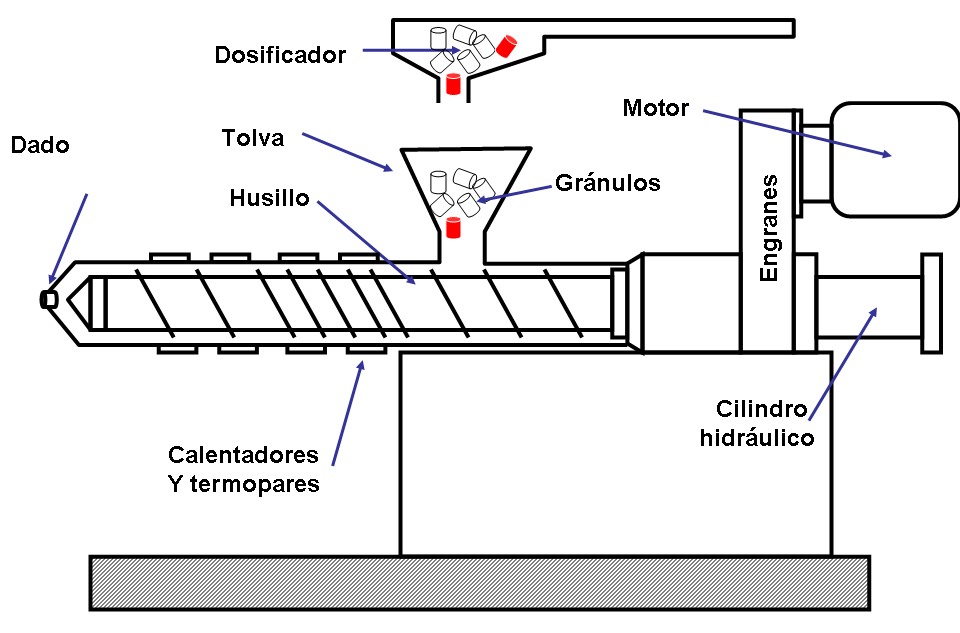
\includegraphics[width=0.6\textwidth]{images/extrusor.png}
    \caption[Esquema básico de una extrusora.]{Esquema básico de una extrusora conformado por: Dosificador, tolva, motor, husillo, calentadores y dado. Fuente \cite{disenoextrusor}}
    \label{fig:estado_extrusora}
\end{figure}

\begin{itemize}
    \item \textbf{Dosificador:} Es el encargado de suministrar el polímero, normalmente en forma de granza, a la tolva garantizando un suministro constante. 
     \begin{figure}[H]
        \centering
        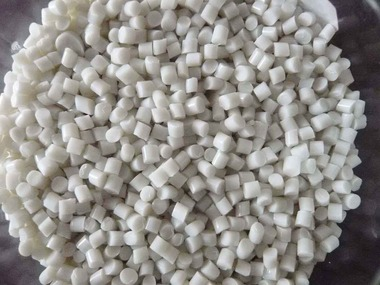
\includegraphics[width=0.4\textwidth]{images/PLA-Pellets.jpg}
        \caption[Pellets de PLA]{Pellets de PLA.}
        \label{fig:Pellets_PLA}
    \end{figure}
    \item \textbf{Tolva:} Depósito en el que cae la granza proveniente del dosificador. Debe proveer un flujo constante al extrusor para evitar cortes en el objeto que se está construyendo. Su diseño es muy importante, y en función del tipo de material que esté suministrando deberá ser de una manera u otra, debido a que el material puede llegar a compactarse en el fondo y no pasar a la extrusora. Algunos modelos de tolva incluyen sistemas de vibración para ayudar a que el material caiga. En la mayoría de los casos y dependiendo del material con el que estemos trabajando, será conveniente que incluya un sistema de secado para eliminar la humedad, puesto que dependiendo de la materia prima puede afectar a la hora de trabajar con el. Por ejemplo, con el uso del PLA es obligatorio su secado antes de la producción.
    \item \textbf{Cilindro hidráulico:} Constituye el cuerpo principal de la extrusora y en su interior está el husillo. Es en este cilindro donde se encuentran las resistencias electricas que aportan la energía calorífica necesaria para fundir el material. La temperatura está registrada a lo largo de las distintas zonas del cilindro, para poder tener un control sobre la temperatura de fusión del material. El cilindro debe estar fabricado con materiales especiales de tal manera, que tenga una buena transferencia de calor y debe ser más duro que el material que se está extruyendo, para lograr una larga duración.
    \item \textbf{Husillo:} Es el elemento más importante de la extrusora y el que determina el grado de calidad con el que la pieza saldrá de la extrusora. Como se aprecia en la figura \ref{fig:estado_husillo} tenemos tres zonas claramente definidas:

        \begin{itemize}
                \item \textbf{Alimentación:} Esta zona, es la encargada de transportar la granza de la tolva al interior del husillo. En la figura podemos ver como los filetes están muy separados del centro del husillo, con el fin de transportar la mayor cantidad posible de material.
                \item \textbf{Compresión:} A medida que entramos en la zona de compresión, los filetes van disminuyendo y se acercan al husillo, con el fin de fundir y homogeneizar el material. Aquí se expulsa el posible aire residual que quede entre la granza.
                \item \textbf{Dosificación:} Conduce el material compactado hacia el dado de la extrusora. Esta zona debe garantizar que el material sale con una temperatura constante y homogéneo.
        \end{itemize}

        \begin{figure}[H]
            \centering
            \begin{subfigure}[b]{0.45\textwidth}
                \centering
                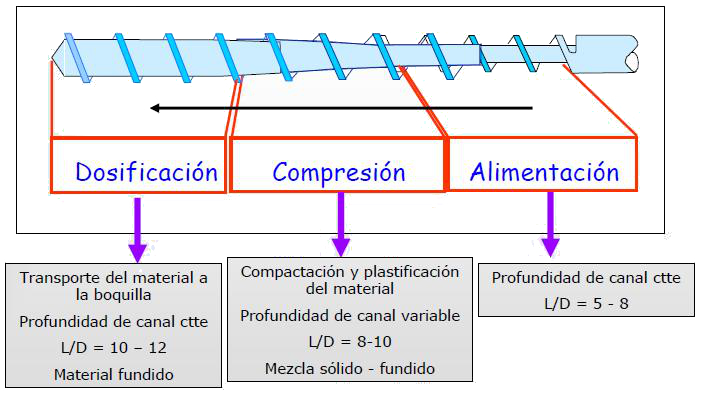
\includegraphics[width=\textwidth]{images/husillo.jpg}
                \label{fig:estado_husillo1}
            \end{subfigure}
            ~
            \begin{subfigure}[b]{0.45\textwidth}
                    \centering
                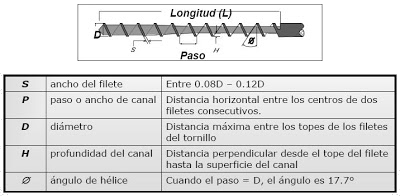
\includegraphics[width=\textwidth]{images/husillo2.jpg}
                \label{fig:estado_husillo2}
            \end{subfigure}
            \caption[Características de un husillo.]{Características de un husillo. En la imagen de la izquierda vemos las distintas zonas del husillo como son: Alimentación, compresión y dosificación. A la derecha, la relación directa que hay entre cada uno de los parámetros que definen el husillo. Fuente  \cite{parametroshusillos}}
            \label{fig:estado_husillo}
        \end{figure}
    \item \textbf{Dado:} En función del dado que se coloque al final de la extrusora, se conseguirá un perfil distinto, en el caso que nos ocupa, el dado tiene un círculo para conseguir la forma de cilindro que deseamos.

        \begin{figure}[H]
                \centering
                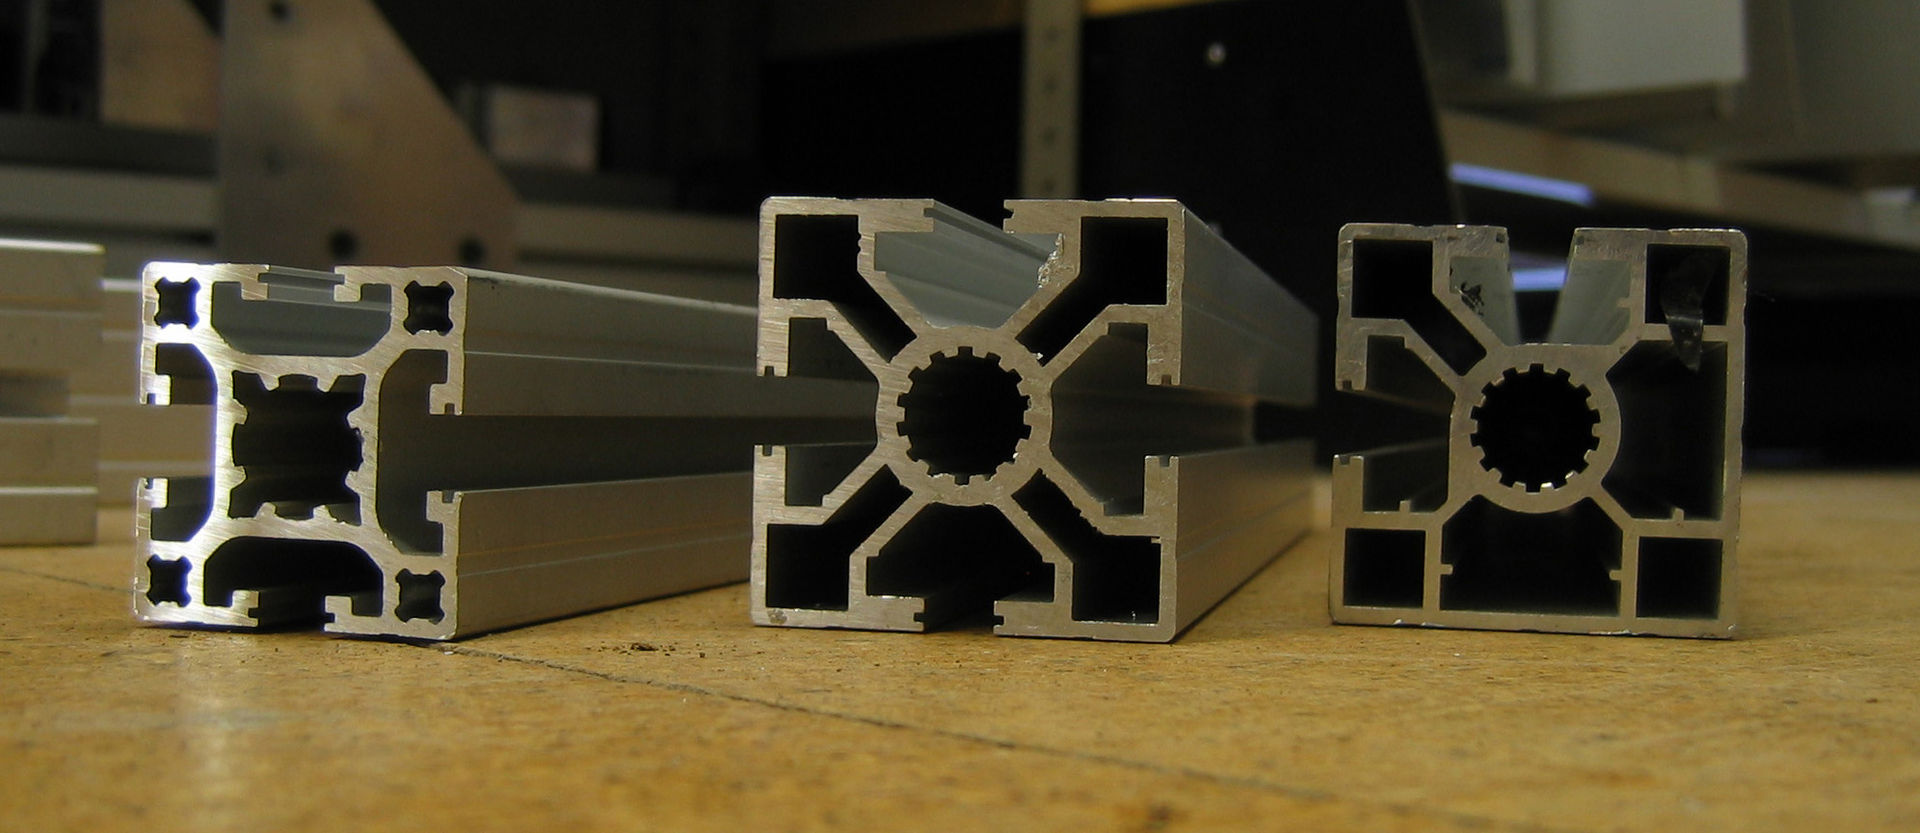
\includegraphics[width=0.5\textwidth]{images/Extruded_aluminium_section.jpg}
                \caption[Distintos ejemplos de extrusión.]{Distintos ejemplos de extrusión con aluminio. Relación de como la forma del dado influye en la forma final del material. Fuente \cite{ejemplosextrusion}}
                \label{fig:estado_ejemplos}
        \end{figure}

\end{itemize}

Hasta ahora, hemos visto como funciona la fabricación aditiva, y los componentes más importantes que lo forman. También la evolución a lo largo de los años de las máquinas que trabajan con esta fabricación. Ahora, vamos a ver como ha sido posible que a día de hoy, podamos tener impresoras 3D a un precio mucho más bajo y competitivo que una impresora profesional.\\

\section{Reprap}
El proyecto Reprap lo inicia Adrian Bowyer y su equipo en 2006 desde la Universidad de Bath \cite{jones2011reprap}. Nace con la idea de facilitar toda la información necesaria para crear y distribuir libremente una máquina de prototipado rápido (ver figura \ref{fig:estado_darwin}).

\begin{figure}[H]
    \centering
    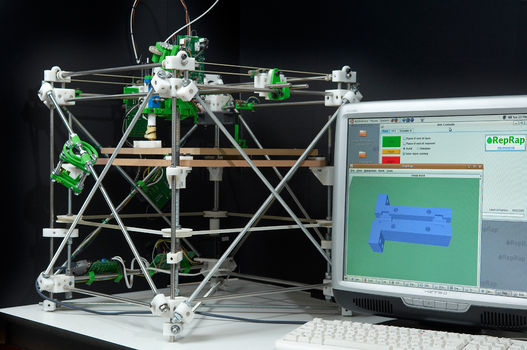
\includegraphics[width=0.6\textwidth]{images/darwin.jpg}
    \caption[Darwin,primera impresora 3D del tipo Reprap]{Darwin,primera impresora 3D del tipo Reprap. Se ve como en su construcción se usan materiales domésticos y como se hace el control desde un ordenador personal.}
    \label{fig:estado_darwin}
\end{figure}

Toda impresora Reprap, es un robot que usa fabricación con filamento fundido para hacer componentes de ingeniería y otros productos desde una variedad de polímeros termoplástico. Reprap es diseñado para que una máquina pueda ser capaz de imprimir un número importante de las piezas que contiene. El resto de piezas, serán piezas fáciles de conseguir en cualquier parte del mundo. De esta manera, se define el término autoreplicante. Toda máquina hecha dentro del proyecto Reprap será libre y open-source así, cualquiera podrá hacerse el número de máquinas que desee, ya sea desde su propia máquina Reprap, como de cualquier otra máquina.\\

Gracias a que Reprap fue liberado con una licencia libre, su expansión en los últimos años ha sido exponencial y ha facilitado que el uso de la fabricación aditiva llegue a las casas, tanto por que está disponible toda la documentación necesaria para realizar una impresora de este tipo desde su web\footnote{\url{http://www.reprap.org}}, como por la distribución a bajo costes de las máquinas.\\

A día de hoy existen más de 50 modelos distintos de impresoras 3D del tipo Reprap, a pesar de que el principio de funcionamiento es el mismo (FDM) cada impresora es distinta y tiene sus ventajas y desventajas. A pesar del alto número de opciones disponibles, el modelo que más éxito ha tenido ha sido el denominado Prusa Mendel.\\

La impresora Prusa Mendel es lanzada en el año 2010 Diseñada por Josef Prusa con tan sólo 20 años, estudiante en la universidad de Praga, Repçública Checa, y basa su diseño en la segunda impresora del proyecto Reprap, la mendel. Como se mencionó anteriormente, toda impresora liberada en Reprap es libre, por ello, Josef Prusa, tomó como base el trabajo que ya había hecho y le añadió algunas mejoras, tales como:

\begin{itemize}
    \item Mucho más sencilla de montar.
    \item Piezas impresas más sencillas.
    \item Fácil de reparar.
    \item Usa mejores componentes lo que hacen que la calidad de impresión mejore.
\end{itemize}

Tras varios años de mejoras e iteracciones en el diseño, Josef liberó en 2012 la prusa I3. La cual introducía un nuevo diseño en la estructura, pasando de usar varillas roscadas a un marco de aluminio que sostenía todo el peso de la impresora, dándole estabilidad y robustez (ver figura \ref{fig:evol_prusa}. Para muchas personas, fue un paso atrás en la idea originaría del proyecto Reprap ya que se intentaba conseguir que la impresora fuera capaz de imprimir al menos el 90\% de sus piezas

\begin{figure}[H]
	\centering
	\begin{subfigure}[b]{0.45\textwidth}
	    \centering
	     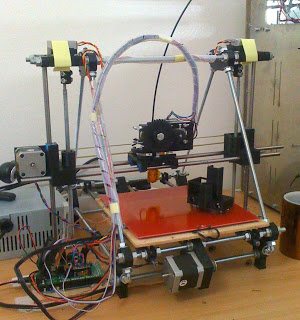
\includegraphics[width=\textwidth]{images/prusa_i2.jpg}
	    \label{fig:prusa2}
	\end{subfigure}
	~
	\begin{subfigure}[b]{0.45\textwidth}
	     \centering
	     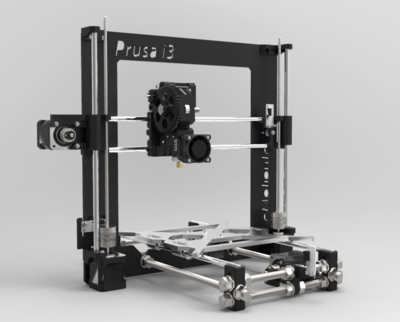
\includegraphics[width=\textwidth]{images/prusa_i3.png}
	    \label{fig:prusa3}
	\end{subfigure}
	\caption[Evolución de las impresoras diseñadas por Josef Prusa.]{En la figura de la izquierda vemos la Prusa I2. En la figura de la derecha la Prusa I3. Tan sólo dos años separan a ambos modelos y se ve una mejora en la simplicidad en el diseño.}
	\label{fig:evol_prusa}
\end{figure}

Pero la facilidad de montaje y que el coste por incluir un marco no incrementaba demasiado el precio final, ha hecho posible que la prusa I3 sea a día de hoy la impresora Reprap más extendida.

\section{Reprap en España}

En Febrero de 2009, Adrian Bowyer impartió una conferencia en Madrid, en el MediaLab Prado, a esa conferencia, asístió Juan Gonzalez Gomez, este era el comienzo de Reprap en España. Como el propio Juan dice en su web \cite{juan1}:

\begin{quotation}
    \emph{
    "He estado siguiendo el proyecto reprap desde hace varios años, pero sólo era una mera curiosidad. Ahora que lo he visto de cerca y he comprobado cómo son las piezas que se pueden fabricar de forma casera, estoy impactado. Estuve durante toda la charla con ese presentimiento de que estábamos al comienzo de algo grande. Es la semilla de un futuro completamente revolucionario”}
\end{quotation}

Desde ese momento, Juan empezó a investigar sobre las impresoras 3D, comprando su propia impresora 3D \cite{juanR1} y empezando a imprimir los primeros Printbot: Robots impresos en 3D, facilitando así el prototipado rápido. Debido a que la impresora que tenía no era muy fiable, pensó en la posibilidad de hacerse su propia impresora Reprap.\\

En ese momento, Juan era profesor visitante en el departamento de ingeniería de Sistemas y Automática de la \textbf{Universidad Carlos III de Madrid} junto con Alberto Valero, ambos, enseñaron a los estudiantes a trabajar con las impresoras 3D. A través de la asociación de robótica de la universidad solicitaron la compra de una impresora 3D de makerbot para que los estudiantes tuvieran acceso a una y pudieran imprimir sus propias piezas, en ese momento comenzó lo que en un futuro sería el proyecto Clone Wars\footnote{http://www.reprap.org/wiki/Proyecto\_Clone\_Wars}.\\


Juan comenzó a trabajar en la construcción de su primera impresora que fue documentando en su propio blog, para transmitírselo a los estudiantes, el 18 de Abril de 2011 se realizó la primera reunión de Clone Wars. Juan documentó todo el proceso de fabricación de una impresora Reprap en la wiki de la asociación de robótica, que más tarde migraría a la web oficial de Reprap, para que de ese modo no estuviera ligado a ninguna universidad y fuera totalmente libre.\\




